\subsection{binocular vision}

We have introduced the imaging principle of binocular vision. Now we start from the left and right images of the dual purpose, calculate the disparity map corresponding to the image, and then calculate the coordinates of each pixel in the camera coordinate system, which will constitute \textbf{point cloud}. In the stereo folder of the code directory in Chapter 5, we have prepared the left and right destination images, as shown in \autoref{fig:stereoExample}. The following code demonstrates the calculation of the disparity map and the point cloud part:

\begin{lstlisting}[language=C++,caption=slambook/ch5/stereoVision/stereoVision.cpp(part)]
Int main(int argc, char **argv) {
    // internal reference
    Double fx = 718.856, fy = 718.856, cx = 607.1928, cy = 185.2157;
    // baseline
    Double b = 0.573;
    
    // read the image
    Cv::Mat left = cv::imread(left_file, 0);
    Cv::Mat right = cv::imread(right_file, 0);
    Cv::Ptr<cv::StereoSGBM> sgbm = cv::StereoSGBM::create(
        0, 96, 9, 8 * 9 * 9, 32 * 9 * 9, 1, 63, 10, 100, 32); // magical parameters
    Cv::Mat disparity_sgbm, disparity;
    Sgbm->compute(left, right, disparity_sgbm);
    disparity_sgbm.convertTo(disparity, CV_32F, 1.0 / 16.0f);
    
    // Generate a point cloud
    Vector<Vector4d, Eigen::aligned_allocator<Vector4d>> pointcloud;
    
    // If your machine is slow, please change the following v++ and u++ to v+=2, u+=2
    For (int v = 0; v < left.rows; v++)
        For (int u = 0; u < left.cols; u++) {
            If (disparity.at<float>(v, u) <= 10.0 || disparity.at<float>(v, u) >= 96.0) continue;
            
            Vector4d point(0, 0, 0, left.at<uchar>(v, u) / 255.0); // The front three dimensions are xyz and the fourth dimension is color
            
            // Calculate the position of the point based on the binocular model
            Double x = (u - cx) / fx;
            Double y = (v - cy) / fy;
            Double depth = fx * b / (disparity.at<float>(v, u));
            Point[0] = x * depth;
            Point[1] = y * depth;
            Point[2] = depth;
            
            Pointcloud.push_back(point);
    }
    
    Cv::imshow("disparity", disparity / 96.0);
    Cv::waitKey(0);
    // Draw a point cloud
    showPointCloud(pointcloud);
    Return 0;
}
\end{lstlisting}

In this example, we call the SGBM (Semi-global Batch Matching)\textsuperscript{\cite{Hirschmuller2008}} algorithm implemented by OpenCV to calculate the parallax of the left and right images, and then transform it into the 3D space of the camera through the geometric model of the binocular camera. . SGBM uses the classic parameter configuration from the network, we mainly adjust the maximum and minimum parallax. The parallax data is combined with the camera's internal parameters and baseline to determine the position of each point in three-dimensional space. In order to save the layout, we have omitted the code to display the point cloud.

\begin{figure}[!t]
    \centering
    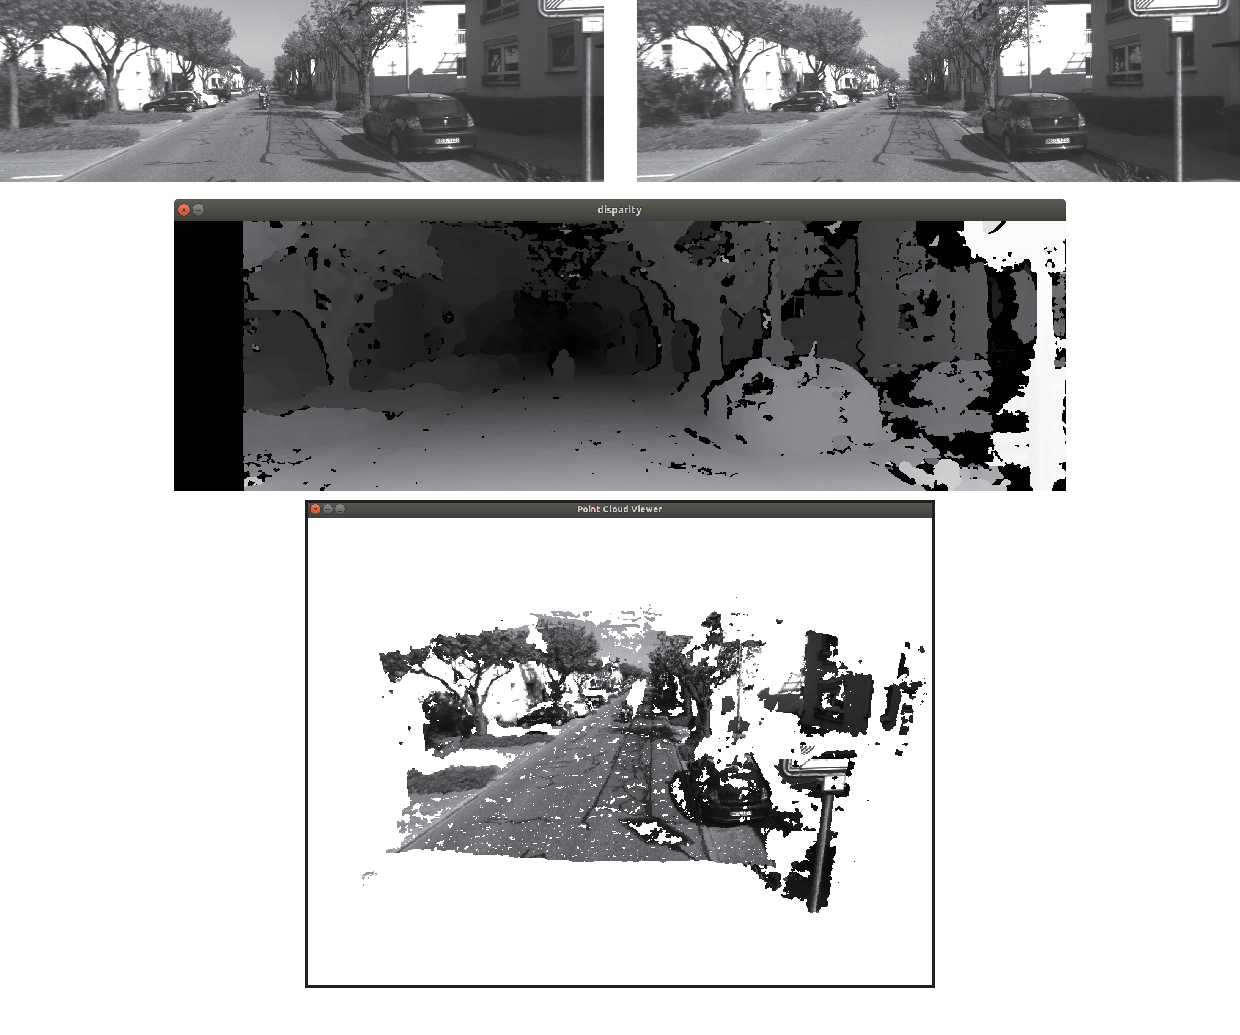
\includegraphics[width=0.9\textwidth]{chapter05/resources/cameraModel/stereoExample.pdf}
    \caption{Example of binocular vision, top left: left eye image, top right: right eye image, middle: SGBM's disparity map, bottom: point cloud image. Note that the left camera sees something that is not seen by the right camera, so the corresponding parallax is empty. }
    \label{fig:stereoExample}
\end{figure}

This book is not intended to introduce a parallax calculation algorithm for binocular cameras. Interested readers can read the relevant reference \textsuperscript{\cite{Scharstein2002, Seitz2006}}. In addition to the binocular algorithms implemented by OpenCV, there are many other libraries focused on implementing efficient disparity calculations. It is a complex and practical topic.